\documentclass{scrartcl}
\usepackage[T1]{fontenc}
\usepackage[utf8]{inputenc}
\usepackage[ngerman]{babel}
\usepackage{amsmath}
\usepackage{amsfonts}
\usepackage{graphicx}
\usepackage{caption}
\usepackage{hyperref}
\begin{document}
\shorthandoff{"}
\paragraph*{Vorbemerkung:}~\\
Da wir mehrere Datenstrukturen bzw. Modelle implementieren, die größtenteils unabhängig voneinander sind, haben wir schon einmal eine initiale voraussichtliche Aufteilung getroffen.
\section{Geometrische Netzwerke (PubWeb)}
PubWeb ist ein Algorithmus zur geometrischen Generierung von Netzwerken. Knoten sind dabei Punkte mit Koordinaten. Knoten, deren Abstand kleiner als eine vorgegebene Länge ist, werden miteinander verbunden. Der triviale Algorithmus (alle Paare testen) braucht quadratische Laufzeit. Zur Beschleunigung sollen nun geometrische Datenstrukturen implementiert werden. Voraussichtlich wird hierfür eine Oberklasse erstellt, um die Modularität zu erhöhen. Für die Datenstrukturen würde sich ein neuer Ordner (z.B. geometric) anbieten.
\subsection{Gitter (Sarah)}
\begin{itemize}
\item Reguläres Gitter: Fest vorgegebene Breite $b$ und Höhe $h$, Zellen in $b \times h$, äquidistante Abstände. Die Raumteilung ist dadurch fest vorgegeben.
\item Adaptives Gitter (z.B. Quadtree): Das Gitter ``baut sich selbst'', da wo mehr Knoten liegen, gibt es eine feinere Unterteilung.
\item Eingaben: Beim regulären Gitter $b$, $h$ (alternativ: Zellengröße) und Weltgröße als Eingaben;  beim adaptiven Weltgröße und Parameter $\gamma \in [0,1]$, der aussagt wieviel Prozent der gesamten Anzahl Knoten in jeder Zelle sein soll (gibt quasi die Granularität an). Alternativ: Pro Zelle ein Knoten. 
\item Schnittstelle: Knoten mit geg. Koordinaten hinzufügen, Knoten in einer Gitterzelle zurückgeben, Knoten in Nachbarzellen zurückgeben (mit übergebener Nachbarschaftsdefinition), Knoten mit Abstand kleiner-gleich übergebenen Wert zu übergebenem Knoten zurückgeben.
\item Geplant: Zweidimensionale Gitter; Erweiterung auf Mehrdimensionalität, falls erwünscht. Es wird sich auf kartesische Gitter beschränkt.
\item Anbindung: Beides in jeweils eigene Klasse. Vermutlich graph/Graph.* für die Knoten. Anbindung an PubWerb: Wie beim kD-Baum.
\end{itemize}

\subsection{kd-Baum (Simon)}
Ein kd-Baum ist eine räumliche Datenstruktur. Der Raum wird hierfür rekursiv jeweils achsenparallel in zwei Teile geteilt, ein (i.A. unbalancierter) Binärbaum entsteht. Meist unterteilt man dabei die Achse mit der größten Ausdehnung. Zur Bestimmung, wo geteilt wird, gibt es mehrere Möglichkeiten. Implementiert werden der Aufbau der Datenstruktur nach dem Objekt-Median und dem räumliche Median, optional je nach Zeitreserven auch nach der Surface-Area-Heuristik (welche den durchschnittlichen Aufwand senken kann). Für die Anbindung an PubWeb wird eine Methode implementiert, die von einem gegebenen Knoten aus die Knoten unter einer bestimmten Entfernung zurückgibt.\\
Benutzt (und wenn nötig angepasst) werden voraussichtlich generators/PubWebGenerator.* und generators/DynamicPubWebGenerator.* für die Anbindung an PubWeb. graph/Graph.* wird für Graphoperationen verwendet. Für den kd-Baum soll eine eigene Klasse neu erstellt werden.

\section{Generierung dynamischer Graphen}
\subsection{Watts-Strogatz (Sarah)}

\begin{itemize}
\item Gegeben: Anzahl Knoten $N$, der mittlere Grad $K$ (gerade natürliche Zahl), ein Parameter $\beta$. 

Es sollen folgende Bedingungen erfüllt werden: $0 \leq \beta \leq 1$ und $N >> K >> \ln(N) >> 1$.
\item Ausgabe: Ein ungerichteter Graph mit $N$ Knoten und $(NK)/2$ über ein randomisiertes Verfahren generierten Kanten.
\end{itemize}

Die Kanten werden nach folgendem Verfahren generiert:
\begin{enumerate}
\item Konstruiere einen ungerichteten Graphen $G=(V,E)$ mit mit $N$ Knoten, in dem jeder Knoten mit $K$ Nachbarn verbunden ist, $K/2$ auf jeder Seite (``regular ring lattice'').
\begin{figure}[h!]
\centering
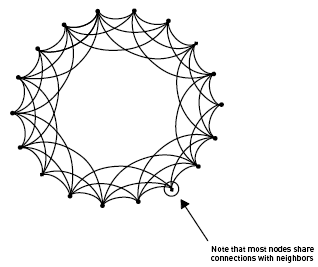
\includegraphics[scale=0.5]{ring.png}
\caption{Ein Ring Lattice, hier allerdings mit schwankender Anzahl Nachbarn. Aber das Prinzip wird deutlich. Bild von \url{http://www.learner.org/courses/mathilluminated/images/units/11/ring.png}}
\end{figure}
Nummeriere die Knoten durch, sodass $V = \{v_0, \ldots, v_{n-1}\}$. Dann gilt
$$\{v_i,v_j\} \in E \Leftrightarrow 0 < |i-j| \mod (n-\frac{K}{2}) \leq \frac{K}{2}$$
\item Betrachte für jeden Knoten $v_i$ jede Kante $\{v_i, v_j\}$ mit $i<j$ und ändere sie mit Wahrscheinlichkeit $\beta$ um. Umändern geht, indem die Kante $\{v_i, v_j\}$ mit einer Kante $\{v_i, v_k\}$ ersetzt wird wobei $k \neq i$ und aus den noch-nicht-Nachbarn von $v_i$ gleichverteilt ein $v_k$ gezogen wird.
\end{enumerate}

\begin{itemize}
\item Vorteile: Kleine-Welt-Eigenschaften wie average path length und high clustering (siehe \url{http://en.wikipedia.org/wiki/Watts_and_Strogatz_model})
\item Nachteile: Fest angegebene Anzahl Knoten, unrealistische Gradverteilung
\end{itemize}

Einbindung in NetworKit:

Ring Lattices in extra Klasse auslagern (machen auch ohne den Rest Sinn), Watts-Strogatz in eigener Klasse in generators, vermutlich werden dieselben Klassen wie bei ForestFire benötigt (außer der Ordner dynamics).

\subsection{Dorogovtsev-Mendes (Sarah)}

\begin{enumerate}
\item Starte mit Dreieck (3 Knoten, 3 Kanten)
\item Füge in jedem Schritt einen neuen Knoten $x$ und zwei Kanten hinzu. Wähle zufällig eine bereits bestehende Kante $\{u,v\}$ und erstelle die beiden Kanten $\{x,u\}$ und $\{x,v\}$.
\end{enumerate}

\begin{itemize}
\item Vorteil: Gibt planaren Graphen zurück, produziert power-low degree distribution (Knoten mit höherem Grad haben bessere Chancen stärker vernetzt zu werden)
\end{itemize}

\begin{figure}[h!]
\centering
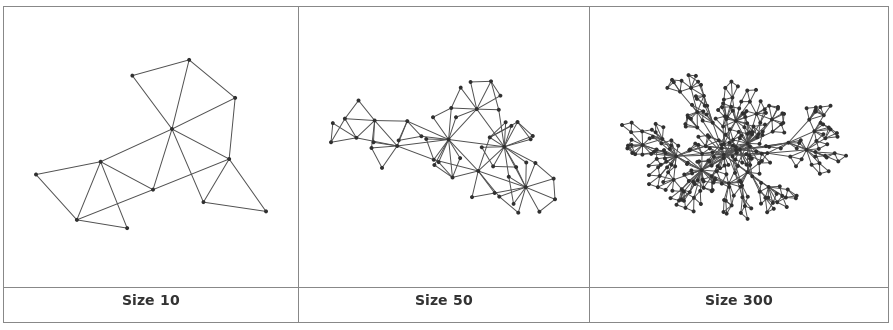
\includegraphics[scale=0.5]{doro.png}
\caption{Sieht dann so aus. Bild von \url{http://graphstream-project.org/doc/Generators/Dorogovtsev-Mendes-Generator_1.0/}}
\end{figure}

Ist wohl schon in NetworKit implementiert (DynamicDorogotsevMendesGenerator.cpp)?

\subsection{Forest Fire (Simon)}
Das Forest-Fire-Modell ist ein randomisiertes Verfahren zur Generierung von Kleine-Welt-Netzwerken, welches also die Bedingungen des Potenzgesetzes und die der kurzen Distanz erfüllt. Die Kantenzahl wächst im Gegensatz zu manch anderen Modellen superlinear in der Knotenzahl. Immer, wenn ein Knoten neu hinzukommt, wird er mit einem zufälligen Knoten ("Botschafter") verbunden. Von diesem aus werden weitere Nachbarn zufällig ausgewählt, die Anzahl wird in Abhängigkeit eines "Entflammbarkeitsparameter" $p$ durch eine geometrische Verteilung mit Mittelwert $\frac{p}{1-p}$ beschrieben (also wird mit Wahrscheinlichkeit $p$ ein zusätzlicher Nachbar gesucht; dies endet beim ersten Fehlschlag). Dies wird rekursiv wiederholt, wobei Knoten höchstens einmal besucht werden. Für den neu hinzugefügten Knoten werden Kanten zu allen so gefundenen Knoten hinzugefügt. Für ungerichtete Graphen ist die Wahrscheinlichkeit $r$ für Rückwärtssuchen irrelevant.\\
Implementiert wird der Forest-Fire-Algorithmus sowie eine Vergrößerung eines bestehenden Graphen mit dem Forest-Fire-Modell.\\
Der Code wird auf dem existierenden, unvollständigen Code in generators/ForestFireGenerator.* aufbauen. Für die allgemeinen Graphoperationen wird graph/Graph.* verwendet. Für den Zufall werden voraussichtlich auxiliary/Random.* sowie graph/Sampling.* benutzt. Da das Modell auch für dynamisch größer werdende Graphen verwendet werden soll, werden wohl auch die Dateien aus dem Ordner dynamics/* benötigt.
\end{document}